\documentclass[12pt]{article}
\usepackage[utf8]{inputenc}
\usepackage{graphicx}
\usepackage{amsmath}
\usepackage{amsfonts}
\usepackage{amssymb}
\usepackage{subcaption}
\usepackage{float}
\usepackage{tikz}
\usepackage{listings}
\usepackage{color}
\usepackage{parskip}
\usepackage{hyperref}
\usepackage{mathrsfs}


\hypersetup{
    colorlinks=true,
    linkcolor=black,
    citecolor=black,
    filecolor=black,
    urlcolor=black
}
\usepackage[left=1in,right=1in,top=1in,bottom=1in]{geometry}
\captionsetup{justification=centering}

\title{Theoretical \& Mathematical Deep Dive: RMMs \& Derivatives}
\author{Alyssa Brittany Chen}
\date{Apr. 10, 2023}

\begin{document}

\maketitle


\tableofcontents

\newpage

\section{Introduction}
Automated Market Makers (AMMs) such as Uniswap and PancakeSwap are decentralized exchanges (DEX) that utilize an algorithmic trading rule that determines how two assets are to be exchanged through two users. These AMM-based DEXs operate primarily through liquidity pools, where liquidity providers (LP) deposit assets into the pool and are rewarded with a fraction of the fees generated on the AMM, usually distributed as LP tokens. This practice of depositing assets to earn rewards is known as yield farming. 

\subsection{Automated Market Makers \& Liquidity}
As traders buy and sell assets on AMMs, insufficient liquidity can lead to high-borrow lending spreads, which can lead to capital efficiency and impermanent loss. (explain why this is bad) 

AMM exchanges are usually based on a constant function– Bancor was one of the first AMM-based DEXs to implement the constant product market maker (CPMM), which is based off the constant product function: x*y=k. This formula accounts the range of prices for two tokens according to the available quantities (liquidity) of each token. When the supply of token X increases, the token supply of Y must decrease, and vice-versa, to maintain the constant product K. 
\begin{figure}[H]
    \centering
    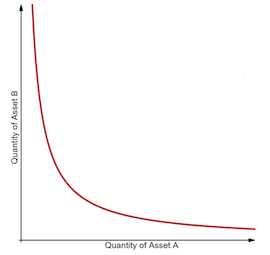
\includegraphics[width=0.5\linewidth]{constant_product.png}
    \caption{Constant Product Function}
    \label{fig:constant_product}
\end{figure}

On the other hand, constant sum market makers (CSMM) follow the formula x+y=k. However, this formula allows arbitrageurs to drain one of the reserves if the off-chain reference price between the tokens is not 1:1, which is why AMMs rarely follow the CSMM model. 
\begin{figure}[H]
    \centering
    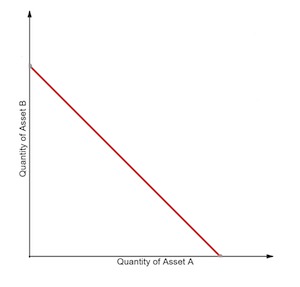
\includegraphics[width=0.5\linewidth]{constant_sum.png}
    \caption{Constant Sum Function}
    \label{fig:constant_sum}
\end{figure}

The final market maker we will cover in this article is the constant mean market maker (CMMM), which enables the creation of AMMs that can have more than two tokens and be weighted outside of the standard 50/50 distribution. For a liquidity pool with three assets, the equation would be the following:
\[
(x*y*z)^{\frac{1}{3}}=k
\]
where the weighted geometric mean of each reserve remains constant (i.e. \href{https://balancer.fi/}{Balancer}).

\section{Limitations of AMMs}
\subsection{Impermanent Loss \& Capital Inefficiency}
Impermanent loss and low capital inefficiency are two limits of AMMs that affect both liquidity providers and traders.

Consider the following example of impermanent loss: After an LP deposits assets into a pool, the price of one of the deposited assets changes significantly compared to the value when initially deposited. As a result, the ratio of assets in the pool will also fluctuate due to arbitrage trading and rebalancing prices that occur with external markets– therefore, in some cases depositing assets could lessen the LP’s positional value, which is the essence of impermanent loss. In other words, this loss is “impermanent” because the loss is recoverable if prices return to its original state when liquidity was initially deposited. On the other hand, the impermanent loss becomes permanent if the LP decides to withdraw their liquidity from the pool at this new price ratio.

Capital inefficiency refers to how effectively liquidity (capital) within a pool is used to facilitate trades without leading to large price impacts. Low capital efficiency indicates that large amounts of liquidity are required to facilitate trades without moving the market price significantly. An ideal DeFi protocol is able to optimally utilize deposited assets to ensure a balanced and efficient market– high spreads is an indication of inefficiency. As a result platforms with high spreads may result in loss of market share over time in comparison to other platforms offering more favorable rates, and this can be unfavorable for LPs because their capital isn't utilized as effectively, leading to lower returns. An example of calculating impermanent loss can be found in ~\ref{subsec:impermanent}.\

Replicating Maker Markets allow users to directly control their impermanent loss by defining a target price around which liquidity will be most concentrated. In the context of traditional markets, this is similar to setting a price in a limit order where a trader specifies the price at which they're willing to buy or sell an asset. RMMs seek to address these limitations via algorithmic strategies to better replicate the ideal liquidity curves and trading functionalities of traditional order book markets, allowing for more efficiency, flexibility, and risk management control.

\section{RMMs Explained}
\subsection{Portfolios \& Continuous Rebalancing}
Simply put, an RMM is an AMM whose portfolio value matches a target payoff. Now, let’s investigate the case of an Uniswap LP, whose value is determined by its underlying assets and their performance over time. When the value of one asset with respect to the other asset changes, the portfolio must be rebalanced such that the composition of value is equally 50-50 in each asset. This rebalancing occurs by arbitrageurs who put one asset in and take another asset out, in order to maintain the pool composition to equal 50-50 value. When the rebalancing occurs, whoever made the trade will have paid a trading fee. This trading fee is earned by all the liquidity providers of the pool. Therefore, as more trades (rebalancing) occurs, their portfolio value will grow over time (the specific fees are determined by the protocol of the specific AMM protocol).

In a Replicating Market Maker, the portfolio is always being rebalanced in a way that it matches a desired payoff. In RMMs, the goal is to replicate or mimic the payoff of certain financial instruments or desired outcome. Unlike traditional AMMs which rely on a predefined mathematical formula to set prices and manage liquidity, RMMs actively manage their portfolios to ensure that the outcome of trading within these markets closely follows a predetermined financial model or payoff structure.

RMMs use algorithms as a mechanism to continuously adjust the composition of their liquidity pools in order to ensure that the value of the pool aligns with the desired payoff structure over time. This process involves algorithmically trading assets within the pool or with external markets to maintain the target allocation and payoff outcome.

\subsection{Replicating Portfolios}

A replicating portfolio (also known as a hedge) is defined as a portfolio of assets that exhibit the same properties as the asset being referenced. In this context, there can be state and dynamic replications. State replication alludes to the portfolio sharing the same cash flows as the reference asset with a stagnant change state, while dynamic replication indicates that the portfolio has a differing cash flow than the reference asset,  but shares the same Greeks (meaning for infinitesimally small changes to underlying market parameters, the asset and portfolio price are altered in the same way). Due to the behaviors of the asset and portfolio’s partial derivatives at a singular point, dynamic replication must occur frequently.

\subsection{Call Options}
A call option in traditional financial markets is a contract between a buyer and seller that gives the right to purchase an asset for a predetermined (strike) price up until an expiration date. This allows the buyer to purchase the stock by exercising the call– however, the buyer does not have the obligation to do so. On the other hand, the seller shorting (selling) the call option has the obligation to sell the asset at the strike price. 

In DeFi, these call options are collateralized to simulate the legally enforceable nature of asset delivery via one part to the other. A covered call occurs when collateral is deposited and the call option is sold. 

In long calls, buyers have the option to openly purchase shares. Purchasing a long call at strike price gives buyers the option to plan ahead. For example, if a tech company frequently has new product launches at around the same time each year, the company’s stock price has the ability to appreciate after the launch. 

Short Calls indicate an open obligation to sell shares. Until the expiration date, the seller is obligated to sell shares of the stock at strike price. Short calls are generally used to increase and boost income. 

Investors in long call options hope for the underlying stock price to rise above the exercise price, and on the contrary, short call investors want the underlying stock price to stay below the exercise price. 

\subsection{RMMs vs. AMMs}

\section{RMM \& CFMM Curves}

\section{Primitive}
Primitive's "RMM-01" is an example of a replicating market maker, built on the idea of a covered call.

\begin{figure}[H]
    \centering
    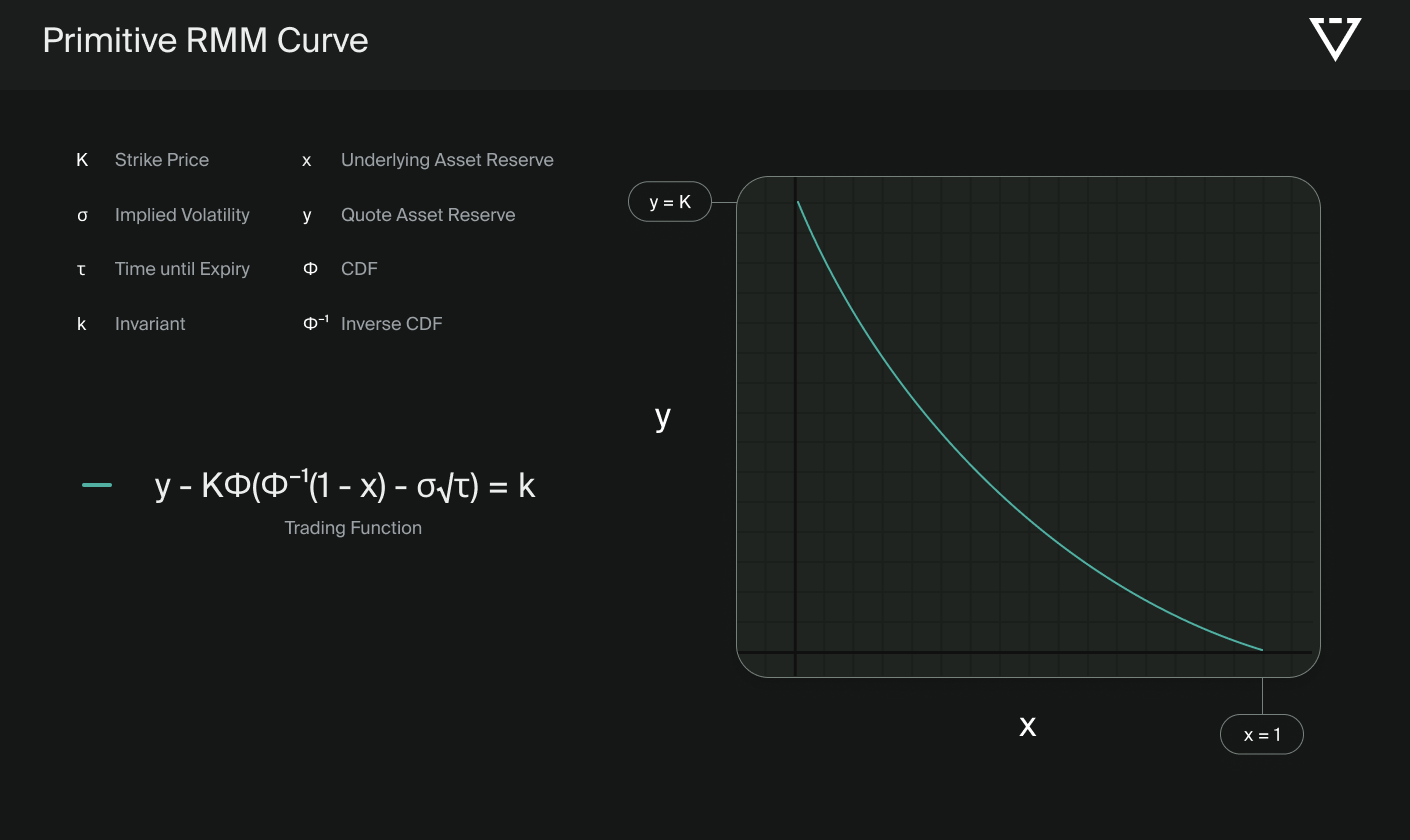
\includegraphics[width=0.8\linewidth]{Primitive.png}
    \caption{Primitive's RMM Curve}
    \label{fig:primitive}
\end{figure}


\section*{Appendix}
\subsection{Impermanent Loss}\label{subsec:impermanent}
\href{https://dailydefi.org/tools/impermanent-loss-calculator/}{Daily Defi} provides an impermanent loss calculator that can be used to visualize the calculations of impermanent loss using Uniswap's constant product formula.
In the following diagram, Token A is initially set to \$150 and Token B is set to \$1. In Future Prices, Token A has increased to \$300 while Token B has remained the same. (The calculator automatically sets a total starting value of \$1000 between the two tokens)
\begin{figure}[H]
    \centering
    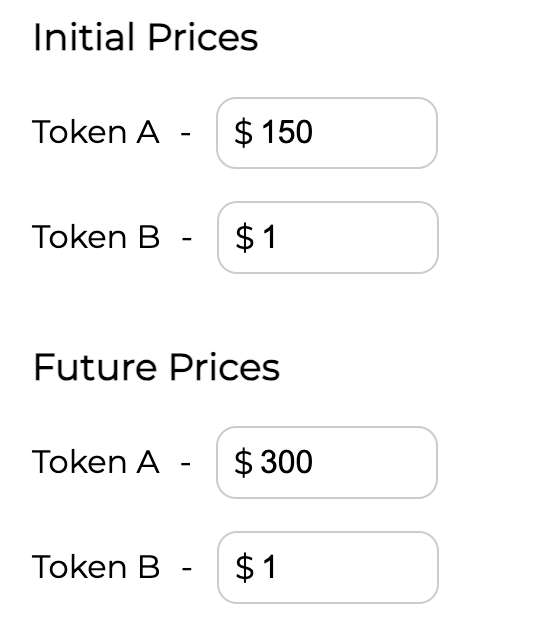
\includegraphics[width=0.4\linewidth]{impermanent_loss.png}
    \caption{Daily Defi's Impermanent Loss Calculator}
    \label{fig:impermanent_loss}
\end{figure}

Below, the results account for the total amount of impermanent loss. The value of Token A and B would be \$1500 if held, and \$1414.21 if provided as liquidity, thereby resulting in an impermanent loss of \$85.79.

\begin{figure}[H]
    \centering
    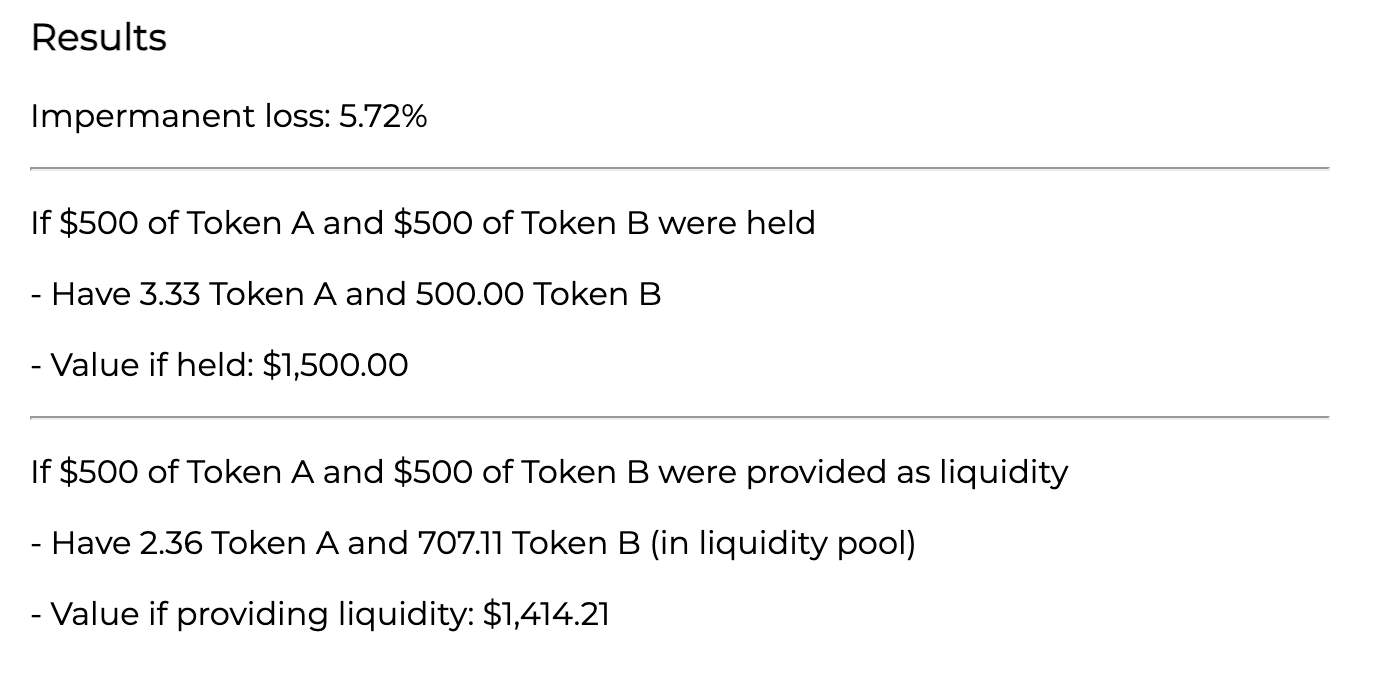
\includegraphics[width=0.6\linewidth]{results.png}
    \caption{Calculations of Impermanent Loss}
    \label{fig:calculations}
\end{figure}

\subsection{Greeks}\label{subsec:greeks}


\end{document}